
\chapter{Estimação, Efeitos Marginais e Econometria Clássica}

Introduzido o conceito de Floresta Aleatória, agora voltamos nossa atenção à Econometria Clássica e seu \texit{workhorse model}, o \textbf{modelo clássico de regressão linear}. Veremos uma maneira de estimar os parâmetros desse modelo, via Mínimos Quadrados Ordinários, como modelos de Floresta Aleatória não têm a mesma interpretabilidade e como podemos contornar essa problemática avaliando o modelo na vizinhança de algumas observações. 



\section{Teoria Clássica de Regressão Linear}

Recuperando o conceito apresentado no início do capítulo interior, um \textbf{modelo} é um mapa entre um espaço de mensuração $\X$ (que neste contexto tem seus elementos chamados de \textbf{variáveis independentes}), com variáveis ditas explicativas do fenômeno representado no espaço de resposta $\Y$. Hayashi CITAR descreve modelos, em um linguajar mais estatístico como (i) um conjunto de restrições sobre a distribuição conjunta das variáveis e/ou (ii) um conjunto de distribuições conjuntas satisfazendo um conjunto de hipóteses. Iremos nos referir às variáveis medidas em $\X$ como \textbf{regressores}. Nesta seção iremos descrever uma família de modelos lineares, suas limitações e virtudes.



\begin{hipotese}[Linearidade]
Nossos modelos $\mathcal{L} : \X \to \Y$ são funções lineares. Nos referimos ao valor da $i$-ésima observação na $j$-ésima variável como $x_{ij}$, sua resposta sendo $y_i$. O termo $\epsilon_i$ é o \textbf{resíduo}, uma variável aleatória que acomodará a parcela não-explicada pelas variáveis em $\X$ da resposta em $\Y$. Se $\X \subset \R^k$ então o vetor de parâmetros que estimaremos será $\boldsymbol{\beta} \in \R^k$ e nossos modelos terão a forma funcional:

\begin{align}
    y_i = \sum_{j = 1}^k \beta_j x_{ij} + \epsilon_i \label{mod_lin}
\end{align}

Linearidade implica que o efeito de uma variação em um regressor particular na resposta não depende do seu nível, nem do de outros regressores. De fato:

\begin{align}
    \frac{\partial y}{\partial x_i} = \beta_i
\end{align}
\end{hipotese}


Essa hipótese pode parecer muito restritiva a princípio, mas não é (tanto). O modelador pode usar de intuição para construir variáveis novas que são funções não-lineares das variáveis mensuradas originalmente. A relação entre salário e experiência ou escolaridade, por exemplo, tem retornos decrescentes. Os primeiros cinco anos no mercado de trabalho contribuem muito mais para um aumento salarial do que os últimos cinco anos de carreira. Essa relação pode ser captada introduzindo um termo com o quadrado da experiência no modelo, por exemplo. 

\begin{exemplo}[Estimando linearmente uma relação não-linear]

Suponha que algum processo de interesse depende de uma variável aleatória $x$ e tenha a seguinte relação: $y(x) = 100 + 5*x - 2x^2$. Observamos $y$ com um erro:

\begin{figure}
    \centering
    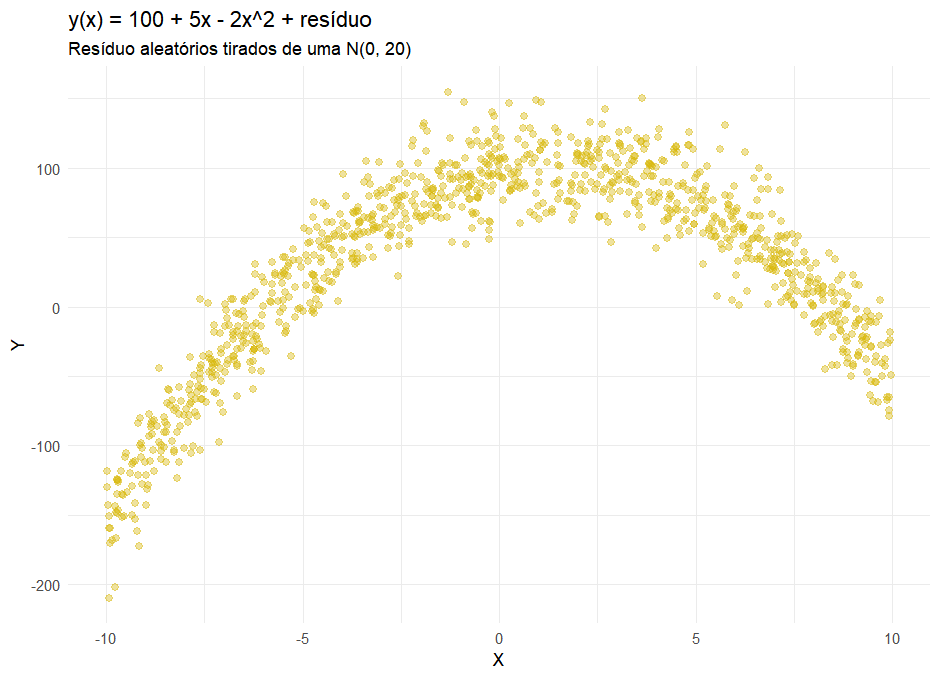
\includegraphics[scale = .55]{imagens/exemplo3_dist.png}
    \caption{Uma amostra simulada do processo. Elaboração própria.}
\end{figure}

\end{exemplo}

Antes de prosseguir é importante apresentar a notação matricial dos modelos lineares. Uma maneira interessante de nos referir aos dados coletados de uma amostra - e como discutiremos estimação isso é importante - é associa-los à uma matriz. Notaremos uma \textbf{matriz de dados} como $\mathbf{X}$ em que $\mathbf{X}_{ij}$ é a medição da $i$-ésima observação na $j$-ésima variável. Também teremos $\mathbf{y}$, o vetor em que a $i$-ésima entrada é a medição da variável resposta da $i$-ésima observação, e $\mathbf{\epsilon}$, o vetor com o resíduo. A partir de agora usaremos $n$ para nos referir ao tamanho da amostra, o número de linhas em $\mathbf{X}$ e $\mathbf{y}$. Reescrevendo a equação \ref{mod_lin} em notação matricial:

\begin{equation}
    \underset{n \times 1}{\mathbf{y}} = \underset{n \times k}{\mathbf{X}} \,\, \underset{k \times 1}{\boldsymbol{\beta}}   + \underset{n \times 1}{\boldsymbol{\epsilon}}
\end{equation}



\begin{hipotese}[Exogeneidade Estrita]
A média condicional do resíduo é nula.

\begin{align}
    \E[\epsilon_i \, | \, \mathbf{X}] = 0
\end{align}

Enquanto função dos dados, a média condicional dos resíduos não necessariamente é linear. Podemos nos livrar desse problema supondo que, no entanto, assume o valor constante de zero. Essa hipótese não é restritiva se, entre as variáveis explicativas, houver uma com valor constante igual à média incondicional dos resíduos. É assim de trás para frente que encontraremos o valor constante do modelo no processo de estimação, inclusive. 

\end{hipotese}

\begin{hipotese}[Ausência de Multicolinearidade]
O posto da matriz de dados $\mathbf{X}_{n \times k}$ é $k$ com probabilidade 1.
\end{hipotese}

Em termos práticos, supomos que as variáveis dadas para um modelo linear são linearmente independentes umas das outras. Se os valores de uma variável podem ser inteiramente determinados pelos valores de outras, a adição dessa variável sobredetermina o sistema. 

Também supomos que nosso modelo erra de maneira consistente:

\begin{hipotese}[Homocedasticidade]
A variância dos erros independe do nível dos regressores:

\begin{align}
    \E[\epsilon_i^2\, |\, \mathbf{X} ] = \sigma^2
\end{align}


\end{hipotese}

Dadas as Condições de Gauss-Markov e uma amostra $(\mathbf{X}, \mathbf{y})$, se $(\mathbf{x}_i, \mathbf{y}_i)$ são i.i.d vale que $ \E[\epsilon_i^2\, |\, \mathbf{X} ] = \E[\epsilon_i^2\, |\, \mathbf{x}_i ]  $.







%%%%%%%%%%%%%%%%%


\section{Estimação de Modelos Lineares por Mínimos Quadrados Ordinários}

\section{Efeitos Marginais em Florestas Aleatórias}






\section{Preenchimento de Suporte}